% !TEX TS-program = XeLaTeX
% use the following command: 
% all document files must be coded in UTF-8
\documentclass{textolivre}
% for anonymous submission
%\documentclass[anonymous]{textolivre}
% to create HTML use 
%\documentclass{textolivre-html}
% See more information on the repository: https://github.com/leolca/textolivre

% Metadata
\begin{filecontents*}[overwrite]{article.xmpdata}
    \Title{Educación de calidad y pandemia: retos, experiencias y propuestas desde estudiantes en formación docente de Ecuador}
    \Author{Marielsa López \sep Mariano Herrera \sep Diego Apolo}
    \Language{es}
    \Keywords{Educación de calidad \sep Pandemia \sep Covid 19 \sep Aprendizaje móvil \sep Conectivismo}
    \Journaltitle{Texto Livre}
    \Journalnumber{1983-3652}
    \Volume{14}
    \Issue{2}
    \Firstpage{1}
    \Lastpage{16}
    \Doi{10.35699/1983-3652.2021.33991}

    \setRGBcolorprofile{sRGB_IEC61966-2-1_black_scaled.icc}
            {sRGB_IEC61966-2-1_black_scaled}
            {sRGB IEC61966 v2.1 with black scaling}
            {http://www.color.org}
\end{filecontents*}

% used to create dummy text for the template file
\definecolor{dark-gray}{gray}{0.35} % color used to display dummy texts
\usepackage{lipsum}
\SetLipsumParListSurrounders{\colorlet{oldcolor}{.}\color{dark-gray}}{\color{oldcolor}}

% used here only to provide the XeLaTeX and BibTeX logos
\usepackage{hologo}

% used in this example to provide source code environment
%\crefname{lstlisting}{lista}{listas}
%\Crefname{lstlisting}{Lista}{Listas}
%\usepackage{listings}
%\renewcommand\lstlistingname{Lista}
%\lstset{language=bash,
        breaklines=true,
        basicstyle=\linespread{1}\small\ttfamily,
        numbers=none,xleftmargin=0.5cm,
        frame=none,
        framexleftmargin=0.5em,
        framexrightmargin=0.5em,
        showstringspaces=false,
        upquote=true,
        commentstyle=\color{gray},
        literate=%
           {á}{{\'a}}1 {é}{{\'e}}1 {í}{{\'i}}1 {ó}{{\'o}}1 {ú}{{\'u}}1 
           {à}{{\`a}}1 {è}{{\`e}}1 {ì}{{\`i}}1 {ò}{{\`o}}1 {ù}{{\`u}}1
           {ã}{{\~a}}1 {ẽ}{{\~e}}1 {ĩ}{{\~i}}1 {õ}{{\~o}}1 {ũ}{{\~u}}1
           {â}{{\^a}}1 {ê}{{\^e}}1 {î}{{\^i}}1 {ô}{{\^o}}1 {û}{{\^u}}1
           {ä}{{\"a}}1 {ë}{{\"e}}1 {ï}{{\"i}}1 {ö}{{\"o}}1 {ü}{{\"u}}1
           {Á}{{\'A}}1 {É}{{\'E}}1 {Í}{{\'I}}1 {Ó}{{\'O}}1 {Ú}{{\'U}}1
           {À}{{\`A}}1 {È}{{\`E}}1 {Ì}{{\`I}}1 {Ò}{{\`O}}1 {Ù}{{\`U}}1
           {Ã}{{\~A}}1 {Ẽ}{{\~E}}1 {Ũ}{{\~u}}1 {Õ}{{\~O}}1 {Ũ}{{\~U}}1
           {Â}{{\^A}}1 {Ê}{{\^E}}1 {Î}{{\^I}}1 {Ô}{{\^O}}1 {Û}{{\^U}}1
           {Ä}{{\"A}}1 {Ë}{{\"E}}1 {Ï}{{\"I}}1 {Ö}{{\"O}}1 {Ü}{{\"U}}1
           {ç}{{\c{c}}}1 {Ç}{{\c{C}}}1
}


\journalname{Texto Livre}
\thevolume{14}
\thenumber{2}
\theyear{2021}
\receiveddate{\DTMdisplaydate{2020}{12}{11}{-1}} % YYYY MM DD
\accepteddate{\DTMdisplaydate{2021}{2}{28}{-1}}
\publisheddate{\today}
% Corresponding author
\corrauthor{Marielsa López}
% DOI
\articledoi{10.35699/1983-3652.2021.33991}
% list of available sesscions in the journal: articles, dossier, reports, essays, reviews, interviews, editorial
\articlesessionname{dossier}
% Abbreviated author list for the running footer
\runningauthor{López et al}
\editorname{Daniervelin Pereira}

\title{Educación de calidad y pandemia: retos, experiencias y propuestas desde estudiantes en formación docente de Ecuador}
\othertitle{Educação de qualidade e pandemia: desafios, experiências e propostas de alunos em formação de professores no Equador}
\othertitle{Quality education and pandemic: challenges, experiences and proposals from students in teacher training in Ecuador}
% if there is a third language title, add here:
%\othertitle{Artikelvorlage zur Einreichung beim Texto Livre Journal}

\author[1]{Marielsa López \orcid{0000-0002-5297-8153} \thanks{Email: \url{marielsa.lopez@unae.edu.ec}}}
\author[3]{Mariano Herrera \orcid{0000-0002-7937-507X} \thanks{Email: \url{marianoherrera@uees.edu.ec}}}
\author[2]{Diego Apolo \orcid{0000-0002-1123-1483} \thanks{Email: \url{diego.apolo@unae.edu.ec}}}

\affil[1]{Universidad Nacional de Educación (UNAE), Carrera de Educación Básica, Grupo de Investigación sobre sistemas educativos (GESE), Cuenca, Provincia de Azuay, Ecuador.}
\affil[2]{Universidad Nacional de Educación (UNAE), Carrera de Educación en Ciencias Experimentales, Grupo de Investigación sobre sistemas educativos (GESE), Cuenca, Provincia del Azuay, Ecuador.}
\affil[3]{Universidad de Especialidades Espíritu Santo, Maestría en Gestión Educativa, Guayaquil, Provincia de Guayas, Ecuador.}

\addbibresource{article.bib}
% use biber instead of bibtex
% $ biber tl-article-template

% set language of the article
\setdefaultlanguage{spanish}
\setotherlanguage{portuguese}
\setotherlanguage{english}

% for spanish, use:
%\setdefaultlanguage{spanish}
%\gappto\captionsspanish{\renewcommand{\tablename}{Tabla}} % use 'Tabla' instead of 'Cuadro'
%\AfterEndPreamble{\crefname{table}{tabla}{tablas}}

% for languages that use special fonts, you must provide the typeface that will be used
% \setotherlanguage{arabic}
% \newfontfamily\arabicfont[Script=Arabic]{Amiri}
% \newfontfamily\arabicfontsf[Script=Arabic]{Amiri}
% \newfontfamily\arabicfonttt[Script=Arabic]{Amiri}
%
% in the article, to add arabic text use: \textlang{arabic}{ ... }

% to use emoticons in your manuscript
% https://stackoverflow.com/questions/190145/how-to-insert-emoticons-in-latex/57076064
% using font Symbola, which has full support
% the font may be downloaded at:
% https://dn-works.com/ufas/
% add to preamble:
% \newfontfamily\Symbola{Symbola}
% in the text use:
% {\Symbola }

% reference itens in a descriptive list using their labels instead of numbers
% insert the code below in the preambule:
\makeatletter
\let\orgdescriptionlabel\descriptionlabel
\renewcommand*{\descriptionlabel}[1]{%
  \let\orglabel\label
  \let\label\@gobble
  \phantomsection
  \edef\@currentlabel{#1\unskip}%
  \let\label\orglabel
  \orgdescriptionlabel{#1}%
}
\makeatother
%
% in your document, use as illustraded here:
%\begin{description}
%  \item[first\label{itm1}] this is only an example;
%  % ...  add more items
%\end{description}
 

% custom epigraph - BEGIN 
%%% https://tex.stackexchange.com/questions/193178/specific-epigraph-style
\usepackage{epigraph}
\renewcommand\textflush{flushright}
\makeatletter
\newlength\epitextskip
\pretocmd{\@epitext}{\em}{}{}
\apptocmd{\@epitext}{\em}{}{}
\patchcmd{\epigraph}{\@epitext{#1}\\}{\@epitext{#1}\\[\epitextskip]}{}{}
\makeatother
\setlength\epigraphrule{0pt}
\setlength\epitextskip{0.5ex}
\setlength\epigraphwidth{.7\textwidth}
% custom epigraph - END


% if you use multirows in a table, include the multirow package
\usepackage{multirow}

% add line numbers for submission
%\usepackage{lineno}
%\linenumbers

\begin{document}
\maketitle

\begin{polyabstract}
\begin{abstract}
La pandemia logró lo que la política pública, los gobiernos o  las iniciativas académicas y sociales no pudieron por varias décadas, que fue llevar a la educación y tecnología a un nivel mundial. Esto ha conllevado muchos retos a las instituciones y a los actores educativos. Brechas digitales y económicas que parecían sobrepasadas o estaban invisibilizadas emergieron, obligando a reflexionar la manera en cómo se puede aportar desde este contexto para lograr una educación de calidad. Por ello, el objetivo de esta investigación fue conocer cuáles son los retos, las experiencias y propuestas en las que se han centrado los estudiantes de una Institución de Educación Superior de Ecuador con el fin de identificar elementos a tomar en cuenta para mejorarla. Para ello, se recurrió a una metodología de enfoque mixto que, mediante revisión bibliográfica y documental, cuestionario y grupo focal, permitió tener una aproximación al fenómeno estudiado. Los resultados de este proceso son relevantes para comprender los escenarios a los cuales se enfrentan los estudiantes: limitaciones en conexiones y dispositivos, percepción de que el aprendizaje no se realiza completamente y la necesidad de recurrir a metodologías que motiven la interacción y participación en clases. Pero también se resaltan propuestas que deben ser tomadas en cuenta para tener una educación de calidad como: potenciar el aprendizaje móvil, fortalecer competencias digitales, conocer las diferentes realidades a las que se enfrentan los estudiantes para adaptar el aprendizaje a ellas y vincular iniciativas desde teorías de aprendizaje emergentes como el conectivismo.

\keywords{Educación de calidad \sep Pandemia \sep Covid 19 \sep Aprendizaje móvil \sep Conectivismo}
\end{abstract}

\begin{portuguese} 
\begin{abstract}
A pandemia alcançou o que políticas públicas, governos ou iniciativas acadêmicas e sociais não conseguiram por várias décadas, que foi levar a educação e a tecnologia a um nível global. Isso trouxe muitos desafios para as instituições e atores educacionais. Lacunas digitais e econômicas que pareciam ser superadas ou invisíveis surgiram, o que nos obrigou a refletir sobre como podemos contribuir a partir desse contexto para o alcance de uma educação de qualidade. Portanto, o objetivo desta pesquisa foi conhecer quais são os desafios, experiências e propostas que os alunos de uma Instituição de Ensino Superior do Equador têm enfrentado para identificar os elementos que devem ser levados em consideração para melhorá-la. Para tanto, utilizou-se uma metodologia de abordagem mista que, por meio de revisão bibliográfica e documental, questionário e grupo focal, permitiu uma abordagem do fenômeno estudado. Os resultados desse processo são relevantes para compreender os cenários que os alunos enfrentam: limitações nas conexões e dispositivos, a percepção de que a aprendizagem não se realiza de forma plena e a necessidade de recorrer a metodologias que motivem a interação e a participação nas aulas. Mas também existem propostas que devem ser levadas em conta para uma educação de qualidade, tais como: promover a aprendizagem móvel, fortalecer as competências digitais, conhecer as diferentes realidades que os alunos enfrentam para adaptar a aprendizagem a elas e vincular iniciativas de teorias emergentes de sistemas de aprendizagem como o conectivismo.

\keywords{Educação de qualidade \sep Pandemia \sep Covid 19 \sep Aprendizagem móvel \sep Conectivismo}
\end{abstract}
\end{portuguese}


\begin{english}
\begin{abstract}
The pandemic achieved what public policies, governments or academic and social initiatives could not for several decades, which was to take education and technology to a global level. This has brought many challenges to educational institutions and actors. Digital and economic gaps that seemed to be overcome or were invisible forced us to reflect on how we can contribute to this context to achieve quality education. Therefore, the objective of this research was to find out what kind of challenges, experiences and proposals students from a Higher Education Institution in Ecuador have faced in order to identify elements to improve it. For this, a mixed approach methodology was used to allow an approach to the studied phenomenon, which was done through bibliographic and documentary review, questionnaire and focus group. The results of this process are relevant to understand the scenarios that students face: limitations in connections and devices, the perception that learning is not fully realized, and the need to resort to methodologies that motivate interaction and participation in classes. But there are also proposals that must be taken into account to have a quality education such as: promoting mobile learning, strengthening digital skills, knowing the different realities that students face to adapt learning for them and linking initiatives from emerging learning systems theories such as connectivism. 

\keywords{Quality education \sep Pandemic \sep Covid 19 \sep Mobile learning \sep Connectivism}
\end{abstract}
\end{english}

% if there is another abstract, insert it here using the same scheme
\end{polyabstract}


\section{Introducción}\label{sec-intro}
A partir de la emergencia sanitaria por la propagación a nivel mundial de la COVID-19, los estados tuvieron que tomar decisiones relevantes en aspectos económicos, sociales y políticos. En poco tiempo, los centros educativos de todos los niveles -inicial, básica, bachillerato y superior- se vieron obligados a adoptar modalidades de enseñanza virtuales.

La suspensión de las clases presenciales obligó a docentes, alumnos y familiares a conectarse de forma virtual, ya sea mediante plataformas en línea o redes sociales, lo que conllevó a una serie de transformaciones con miras a brindar una educación de calidad.

En primer lugar, se tuvo la necesidad de adecuarse y aprender sobre la marcha. Los docentes debieron adaptarse a Plataformas como Moodle y Zoom, en la mayoría de los casos, sin formación previa y sin la familiaridad que aporta el uso cotidiano. Esto fue, sin duda, causa de angustia y estrés para docentes, alumnos y seguramente también para sus familiares. Así pues, el \textcite{laboratorio_latinoamericano_de_evaluacion_de_la_calidad_de_la_educacion_[llece]_sistemas_2020} de la \textcite{unesco_bid_2020} y otras instancias nacionales de diversos países han reportado estudios sobre las afectaciones que esto ha causado \cite{unesco_bid_2020}.

Una segunda implicación es que el dominio relativo aunque cada vez mayor de las plataformas por parte de sus nuevos usuarios -docentes y alumnos- no garantiza un uso adecuado de la tecnología para un nivel de aprendizaje satisfactorio, lo que afecta directamente a la percepción de la calidad de esta. 

En diálogo con lo anterior, un análisis de los temas pendientes en educación y tecnología a partir del 2007 en Ecuador, \textcite{apolo_pending_2020a} enfatizan que, si bien es cierto se han realizado avances en lo referente al uso de la tecnología digital, se identificaron tres focos que no han permitido un desarrollo integral: 1) poca consecución de objetivos planteados, 2) carencia de competencias digitales en actores educativos y 3) formación centrada en un manejo artefactual de dispositivos. Si bien es cierto la dotación de conexiones y dispositivos es un paso inicial, en más de 10 años se debió haber planteado una política integral de inclusión digital que trascendiera planes aislados o programas desarticulados.

La tercera implicación es que tanto el uso de la tecnología como la pedagogía adaptada a estos espacios tienen como condición un acceso universal a Internet y que los dispositivos estén disponibles para los estudiantes y docentes, permitiendo fortalecer los aprendizajes sincrónicos o asincrónicos. Pero lamentablemente esto no se ha cumplido debido a que la pandemia profundizó aún más las brechas digitales y económicas existentes.

En este sentido, la relación pobreza y educación dejó en evidencia que una gran cantidad de estudiantes no pudieron continuar con su formación. Según la Organización de las Naciones Unidas [ONU] en Ecuador se estimaba que (\Cref{Fig01}):

\begin{figure}[htbp]
 \centering
 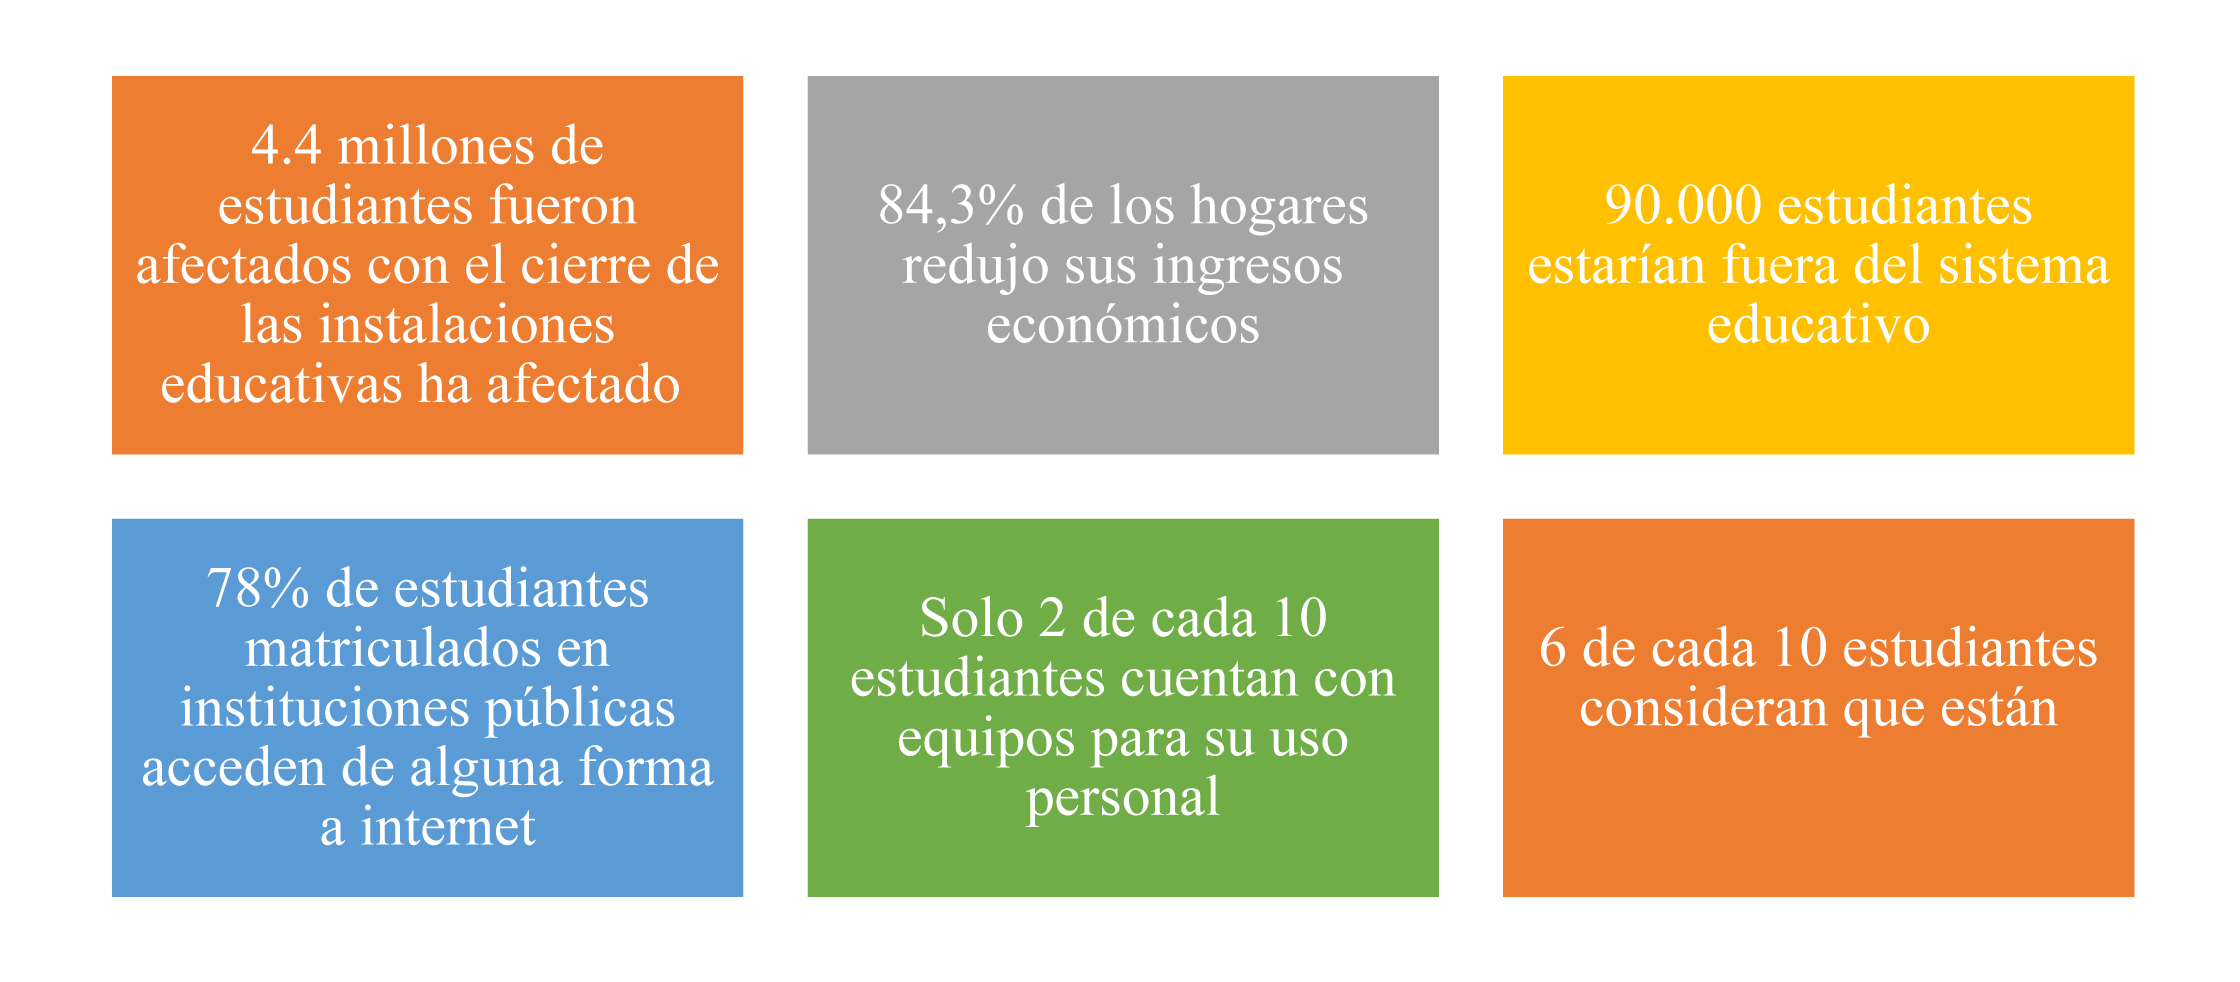
\includegraphics[width=0.85\textwidth]{Fig01.jpg}
 \caption{Datos sobre pandemia en Ecuador.}
 \label{Fig01}
 \source{Elaboración propia a partir de la \textcite{organizacion_de_las_naciones_unidas_[onu]_priorizar_2021}.}
\end{figure}

Estos datos son fundamentales para comprender la magnitud de la afectación no solo económica que vivieron los países, sino también, mostrando un gran retroceso en la consecución de los Objetivos de Desarrollo Sostenible [ODS] en su componente 4, relacionado a la educación de calidad \cite{organizacion_de_las_naciones_unidas_[onu]_objetivos_2012}. Esto debido a que pese a todos los esfuerzos de las instancias pertinentes, los aprendizajes no están cumpliendo del todo su cometido en el caso de quienes sí pueden asistir a las clases. A partir de esto, \textcite{miguel_roman_educacion_2020} menciona que también en México se han esforzado por plantear estrategias para fortalecer la educación tomando en cuenta la brecha digital existente; pero el principal reto es el poco desarrollo de competencias digitales que estudiantes y docentes han demostrado, lo que afecta directamente a su calidad.

Por ejemplo, en el caso de los niveles de educación inicial, básica y bachillerato se ha estimado que la pérdida de aprendizajes es de 40 \%; es decir, los alumnos están aprendiendo máximo 60 \% de lo que hubieran aprendido si estuvieran en clases presenciales \cite{unesco_bid_2020}. En el caso de Ecuador, tanto las evaluaciones nacionales como internacionales indicaban que antes de la pandemia los aprendizaje de los alumnos no eran satisfactorios, aunque en los últimos años se han incrementado. Es importante recalcar que para la educación superior no existen datos acerca de las pérdidas en niveles de aprendizaje, pero por lo encontrado en este estudio y en otros similares, puede inferirse que la situación no es mucho mejor.

\textcite{diaz_quinones_pandemia_2020} en Cuba reportan que para fortalecer la calidad educativa en este contexto es necesario adecuar los planes de estudio y formas organizativas a los contextos de estudiantes, buscando siempre la articulación entre contenidos, disciplinas y asignaturas. Sin descartar tampoco lo que \textcite{silas_casillas_docente_2020} observan en su estudio desarrollado a partir de la percepción de docentes de varios países de Latinoamérica, que el impacto ha sido grande para ellos y para los estudiantes debido a que más del 85 \% únicamente recibían clases presenciales en Instituciones de Educación Superior.

Es así como la emergencia no solo transformó la cotidianidad sino también, cómo los actores educativos enseñan y aprenden. La premisa -modelos educativos del siglo XIX, docentes del siglo XX y estudiantes del siglo XXI- eclosionó vertiginosamente. En la mayoría de los casos los modelos educativos y currículos de instituciones educativas se centran en el constructivismo como teoría de aprendizaje preferente frente al conductismo de la educación tradicional. 

Si se considera que a partir de los años 80 hasta la actualidad, la teoría constructivista ha dominado los discursos pedagógicos en particular, en España y en Latinoamérica, las universidades que forman docentes han intentado articular estas líneas a sus modelos pedagógicos. Específicamente en Ecuador, el currículo de los niveles de educación obligatoria \cite{ministerio_de_educacion_de_ecuador_curriculo_2016} se declara constructivista. Podría estimarse que la mayoría de los docentes que actualmente ejercen profesionalmente en el sistema educativo ecuatoriano, han recibido una formación con este enfoque. 

Posteriormente se han promulgado teorías educativas emergentes que corresponden a las propuestas de \textcite{bonilla-guachamin_dos_2020} quien plantea la necesidad urgente de repensar estos modelos pedagógicos que estuvieron presentes por muchos años en los diferentes niveles educativos. Así pues, los diferentes estudios y los retos enunciados requieren identificar convergencias entre la manera en que interactúan los actores en los actuales escenarios y las teorías. 

Hace más de una década surgieron algunas teorías de aprendizaje que intentaban adecuarse a lo que las sociedades vivían en la educación. \textcite{siemens_connectivism:_2004, siemens_connectivism:_2005} presentó el conectivismo como una teoría de aprendizaje para la era digital. Cabe destacar que esta ha tenido tanto seguidores como detractores, pero algo que no puede negarse es que en pandemia muchos de sus postulados pudieron ayudar a estos problemas que vivieron instituciones, docentes y estudiantes (\Cref{Fig02}).

\begin{figure}[htbp]
 \centering
 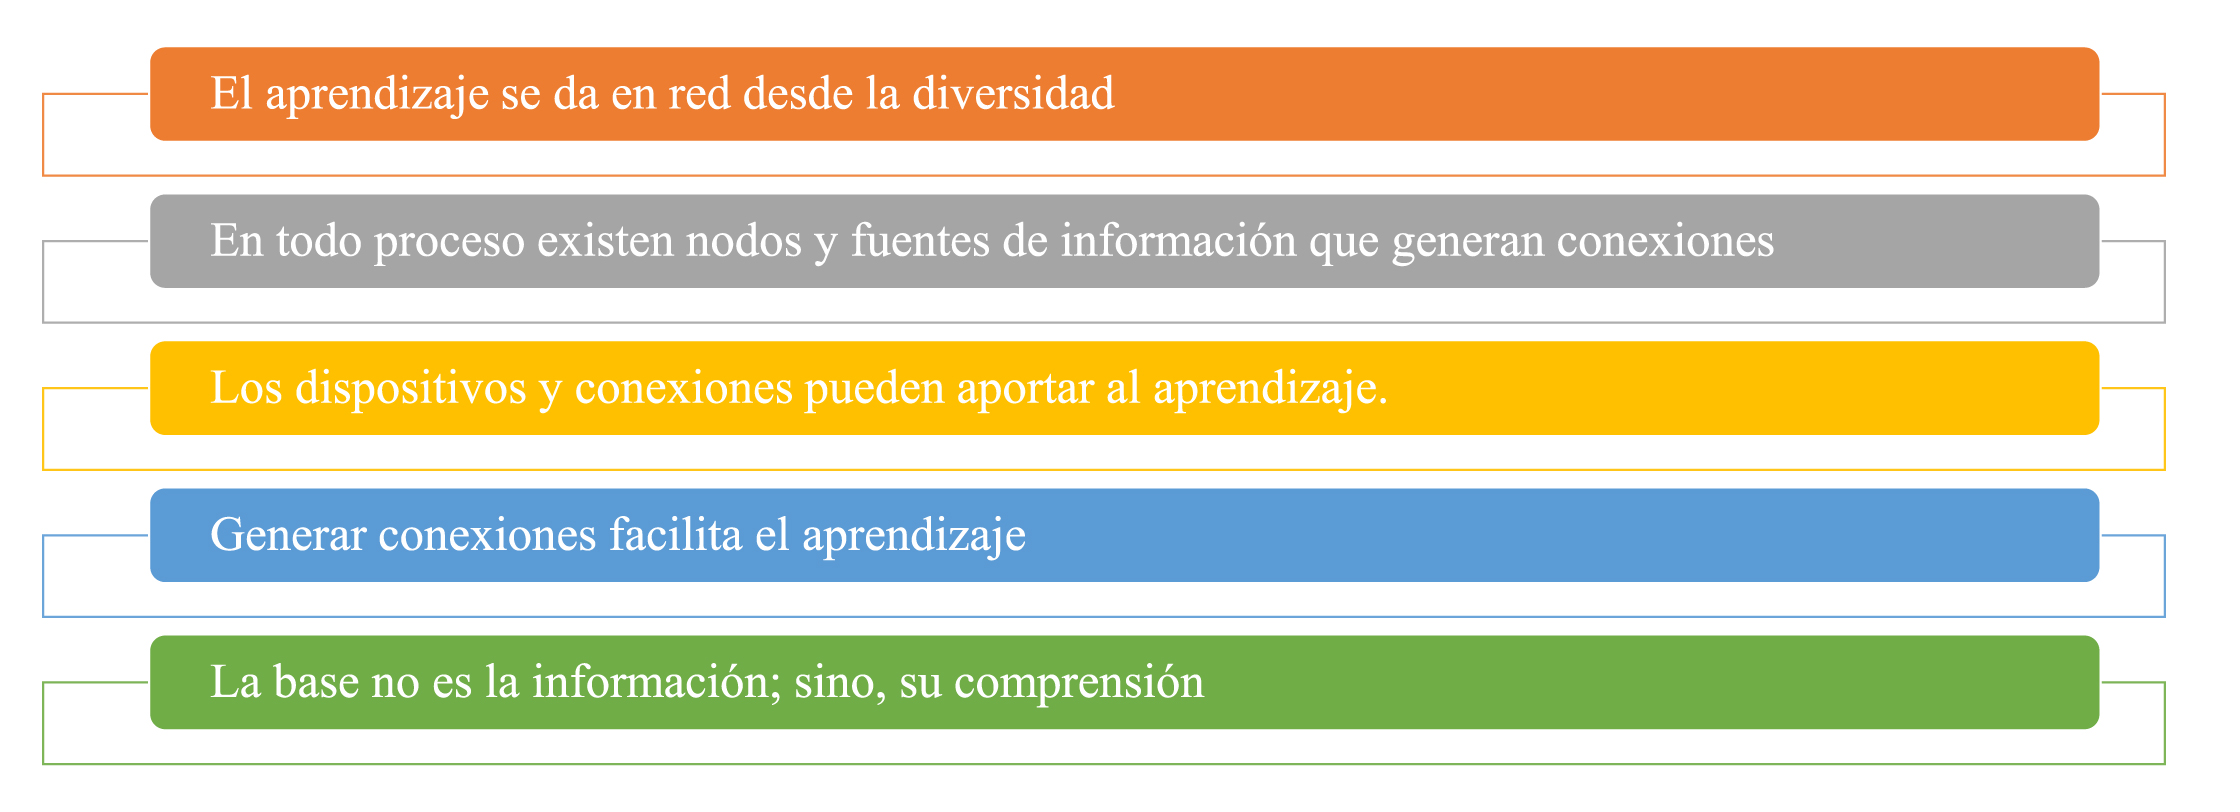
\includegraphics[width=0.85\textwidth]{Fig02.jpg}
 \caption{Ideas sobre conectivismo.}
 \label{Fig02}
 \source{adaptación de \textcite{gutierrez_conectivismo_2012}.}
\end{figure}

Por tanto, en el contexto actual surge la necesidad de aprovechar el uso de plataformas digitales y redes sociales con fines educativos, lo que hubiese permitido llegar a estudiantes que por poca capacidad de conexión no han podido continuar con sus estudios, es más, se estima que “de 1.4 millones de estudiantes de Sierra-Amazonía, se perdió el contacto con 17.754, que equivale al 1.3 \%” \cite[párr. 6]{el_comercio_rastro_2020}. Esto evidencia esa falta de operacionalización desde la política pública y el diálogo con este modelo emergente. 

El objetivo de este estudio fue describir el contexto social y las condiciones que caracterizan el proceso de aprendizaje de estudiantes en formación inicial como docentes de una Institución de Educación Superior de Ecuador, con el fin de conocer cuáles son los retos, las experiencias y propuestas a los que se han visto enfrentados.

\section{Materiales y métodos}\label{sec-normas}
El desarrollo de esta investigación partió de un enfoque mixto de alcance descriptivo exploratorio, tomando en cuenta aportes de diferentes autores para la construcción de instrumentos \cite{restrepo_mesa_metodos_2020, pereira_perez_disenos_2011, hernandez_sampieri_metodologiinvestigacion_2014}. En cuanto al abordaje cuantitativo, el mismo se construyó con el fin de aproximarse a una mayor cantidad de informantes y a partir de esos datos de contexto identificar las experiencias y los usos que dan a dispositivos y conexiones. A continuación se desarrolló una aproximación cualitativa mediante el desarrollo de un grupo focal que permitió conocer con mayor profundidad los retos y las propuestas que han tenido que enfrentar los estudiantes.

Se contó con la participación de estudiantes de los tres primeros ciclos de la carrera de educación en ciencias experimentales de la Universidad Nacional de Educación (UNAE) de Ecuador, durante el periodo SI2020-SII2020, lo que arrojó un total de 176 informantes con una participación equitativa entre hombres y mujeres, provenientes de 7 provincias del país. Posterior al análisis de los datos que emergieron desde el cuestionario, se procedió a realizar un grupo focal que estuvo compuesto por 3 estudiantes hombres y 3 mujeres seleccionados a partir de los usos y las experiencias que han realizado en temas educativos a lo largo del tiempo en pandemia. 

Para el análisis de los datos cuantitativos, se recurrió a estadística descriptiva, permitiendo identificar mediante el cruce de variables datos relevantes para comprender el contexto estudiado \cite{ordonez_pinzon_estudio_2006}. En cuanto a la información que surgió desde la narrativa del grupo focal se procedió al análisis interpretativo como método para identificar las percepciones de los participantes \cite{onwuegbuzie_marco_2011}. Se resalta la importancia de comprender a la investigación como un proceso donde, en un primer momento, se realizó la aplicación de un instrumento y su análisis,  para posterior a ello reforzar el siguiente instrumento con la miras a la triangulación en cuanto a la presentación de resultados. 

\section{Resultados y discusión}\label{sec-conduta}
En este espacio, se presentarán los análisis de resultados a partir del diálogo entre datos, aportes teóricos y otras investigaciones. Se ha articulado una serie de epígrafes que permitirán dar el paso a la comprensión del fenómeno analizado. 

\subsection{Retos en cuanto al uso de conexiones y dispositivos}\label{sec-fmt-manuscrito}
Se puede mencionar que el 91,5 \% de los estudiantes encuestados afirma que tiene posibilidades de acceder a internet y recibir clases en línea, mientras que 8,5 \% no tiene acceso. Esto contrasta con la información del \textcite{instituto_nacional_de_estadisticas_y_censos_de_ecuador_[inec]_encuesta_2020} según la cual el 45,5 \% de los hogares en Ecuador tiene acceso a internet. Al detallarse la información, se constata que, en el medio urbano la proporción de hogares con acceso a Internet sube a 56,1 \%, cabe evidenciar que los informantes se encuentran en zonas rurales y urbanas. 

Cuando se observan estos datos según los cuales el acceso a Internet es masivo en la población de la muestra, podría pensarse que se trata de una franja que pese a pertenecer a los Quintiles más bajos -1 y 2- han logrado, mediante diferentes formas, mantener la conexión a internet. Sin embargo, al profundizar en las opiniones, se determina que el acceso a Internet parece ser alto, pero existe una dificultad que debe tomarse en cuenta: la estabilidad de las conexiones. En efecto, los estudiantes comentan que prevalece una mala calidad (GRUPO FOCAL, 2021). Esto coincide con otras investigaciones como las propuestas por \textcite{pericacho_experiencias_2020} realizadas en España, enfatizando que uno de los principales impedimentos es la estabilidad en conexiones para la educación en línea.

De igual manera, el 92,6 \% de informantes se conecta entre 5 y 7 días a la semana. Un punto interesante para el análisis es conocer que el 71 \% lo hace desde Wifi propio y el 22.7 \% comparte la red con familiares o vecinos. En cuanto a las horas de conexión, 51,7 \% de los estudiantes afirma que se conecta principalmente entre 4 y 7 horas al día. Cabe indicar que si se conectan más de dos personas a la vez, llueve o se vive en una zona montañosa, la conexión se cae. También la red empeora a determinadas horas del día, básicamente en las mañanas debido a que es el horario en que más personas se conectan para trabajar o estudiar “no es problema de falta de computador sino del internet, se cuelga si se conectan dos personas a la vez” (P1, GRUPO FOCAL, 2021).

Hay estudiantes que comparten el internet con todas las familias de un edificio de tres pisos. Por ejemplo, una estudiante cuenta que vive en el mismo edificio que una maestra que imparte clases a sus alumnos a través de la plataforma Zoom durante toda la mañana. Mientras la profesora trabaja, el resto del edificio tiene grandes dificultades de acceso. Los demás vecinos deben turnarse para acceder a la red o lo hacen por sorteo (P4, GRUPO FOCAL, 2021). Otra estudiante comparte la red con todos los clientes del restaurante de su familia. La velocidad de Internet en su caso es mínima, porque además también se usa en su casa (P5, GRUPO FOCAL, 2021).

De manera general, se debe destacar que familias numerosas también se ven obligadas a establecer prioridades para el uso de la red. En una familia donde viven 3 adultos y 4 niños en edad escolar se le asigna la única computadora de la familia a la persona de debe asistir a alguna de las asignaturas más importantes. Los demás miembros de la familia utilizan sus dispositivos móviles, pero la velocidad es baja y las interrupciones en la conexión son frecuentes.

Según el \textcite{instituto_nacional_de_estadisticas_y_censos_de_ecuador_[inec]_encuesta_2020}, en Ecuador solo 23 \% de las familias dispone de un computador en su residencia. De tal manera que, el 77 \% de la población en general no cuenta con ordenadores en sus hogares, retomando aportes de la \textcite{organizacion_de_las_naciones_unidas_[onu]_priorizar_2021} solo 2 de cada 10 estudiantes cuentan con equipos para su uso personal. Esta particularidad hace que sea imprescindible encontrar otras maneras de acceder a Internet. 
Esto en relación con lo indicado por los informantes quienes principalmente se conectan desde un celular. Esto concuerda con datos del \textcite[p. 19]{instituto_nacional_de_estadisticas_y_censos_de_ecuador_[inec]_tecnologias_2019} donde se menciona que el “teléfono celular activado alcanzó 59,9 puntos a nivel nacional, 65,6 puntos en el área urbana y 47,6 puntos en el área rural”. El porcentaje de personas que cuenta con un teléfono inteligente activado aumentó en 6.6 puntos, mientras que el uso en hogares de computador de escritorio disminuyó 1.2 puntos y el acceso a computador móvil aumentó 4.3 desde el 2012. 

Sin embargo, estudios como el realizado por \textcite[p. 213]{roig-vila_comunicacion_2021} demuestran que la mala conexión independientemente del dispositivo influye en el aprendizaje o participación: “lo cierto es que también con los compañeros, los problemas de carácter técnico parecen haber entorpecido la comunicación, especialmente la mala conexión a Internet y los problemas de audio”. Es así pues, relevante que los responsables de las políticas públicas comprendan que para una educación de calidad, no puede separarse la dotación de conexiones a la de dispositivos. 

Esto permite suponer que las computadoras están siendo sustituidas por los dispositivos móviles y que los estudiantes acceden a las clases virtuales a través de ellos.  Por esto es fundamental desarrollar estrategias y al momento de realizar actividades pensar en estudiantes que se conectan mediante móviles, debido a que éstos adquieren una importancia capital para el acceso a Internet y a las clases virtuales. Adicionalmente, en el caso de los estudiantes entrevistados, el problema radica también en la cantidad de personas que comparten el ordenador. En efecto, 82,4 \% de ellos debe compartir el computador con otros miembros de la familia y solo un 17,6 \% dispone de uno de uso exclusivo:

\begin{quote}
    Somos una familia de 4 niños y un adulto y todos asistimos a clases por internet y tenemos una sola computadora. La computadora la usa uno de los niños que tiene problemas de la vista. Todos los demás utilizamos nuestros celulares. Solo en la noche puedo tener la computadora para mi sola y aprovecho para hacer los deberes con los compañeros hasta la madrugada (P4, GRUPO FOCAL, 2021).
\end{quote}

La masiva penetración de los celulares en la población y la poca disponibilidad de computadoras por persona tienen como consecuencia que el teléfono móvil esté sustituyendo a los ordenadores como dispositivo de acceso a internet. Esta información es sumamente útil para poder organizar un plan de educación de calidad virtual a nivel nacional partiendo del uso de estos dispositivos. Esto debería indicar la necesidad de considerar estrategias adaptadas a la enseñanza a través de aplicaciones de teléfonos móviles. Con respecto a esto, \textcite{martinez_uso_2020} encontraron que los estudiantes en España emplean sus celulares para entrar a sus clases virtuales y mencionaron a Netflix como una estrategia para aprender idiomas.

En vista de las dificultades para acceder a las clases a través de ordenadores al tener que compartir computadoras por varios miembros de la familia y la baja calidad de internet por su uso intensivo, los estudiantes encuestados han comenzado a utilizar plataformas diferentes a Zoom y a Moodle para acceder al conocimiento. Afirman que “Zoom es muy pesado y se corta mucho (…) si se prende la cámara, el zoom te bota de la clase (…) Moodle depende de que el profesor sea ordenado y algunos no lo son, a veces es difícil encontrar las cosas” (GRUPO FOCAL, 2021). 

En efecto, el 69 \% de los informantes afirma que ha adquirido sus conocimientos en internet y recursos digitales por sí mismo, mediante páginas y tutoriales. Solo el 14,5 \% sostiene que ha aprendido en la institución educativa y 8,5 \% con ayuda de amigos. En este enfoque sobresalen los conocimientos informales donde en pandemia definitivamente YouTube se ha vuelto la principal plataforma para los aprendizajes. 

En consecuencia, para fortalecer una educación de calidad es relevante motivar a que los estudiantes realicen sus propias búsquedas sobre los temas tratados en clase. Según \textcite{cobo_aprendizaje_2011} la construcción de aprendizajes invisibles puede aportar a ámbitos formales o \textcite{mendoza_castillo_lo_2020} quien comenta que las emociones juegan un papel importante para aprender en este contexto. En este caso los estudiantes utilizan Youtube y organizan grupos de WhatsApp y Facebook para ayudarse entre ellos y compartir el conocimiento: “en Youtube explican mucho mejor, Julio el profe, Alex el profe (…) los docentes graban las clases pero yo no pierdo el tiempo viendo eso. Veo el tema y me voy a Youtube o a Wikipedia Académica” (GRUPO FOCAL, 2021).

Adicionalmente, conforman comunidades de aprendizaje mediante grupos de Whatsapp para compartir información, organizar los deberes y ayudarse entre ellos: “los deberes los dividimos entre las personas del grupo, tú haces esto, tú esto y así” (P6, GRUPO FOCAL, 2021). Esto ha sido una tónica en varios países como se observa a partir de los estudios de \textcite{baptista_lucio_encuesta_2020} en México donde esta plataforma se ha convertido en un espacio para entregar tareas y mantener comunicación.

En tal sentido, se observa el incremento de estrategias de aprendizaje de los alumnos centradas en el trabajo colaborativo en grupos, colaboración, compartir equipos, división de tareas. Así también, es fundamental el seguimiento desde instituciones educativas para conocer la manera en que se usan las plataformas oficiales para fortalecer y acercarse a las realidades de los estudiantes, quienes prefieren migrar a plataformas no oficiales que cumplen con el papel de ayudar a la autoformación y la co-formación. 

Consideran también, que estas plataformas abiertas son de fácil navegabilidad, con estrategias especializadas en la formación en línea y con la posibilidad de acceso ininterrumpido a cualquier hora del día o de la noche, dependiendo de cuando ellos puedan tener la posibilidad de conectarse. Si bien es cierto que se debe responder al uso de espacios institucionales, es necesario también que se puedan complementar los entornos virtuales de aprendizaje con plataformas digitales y redes sociales que se adecúen al contexto de los estudiantes \cite{perez-gomez_educarse_2012}.

La pandemia ha obligado a las familias a organizarse de una manera diferente alrededor del teletrabajo y la educación virtual. El hecho de que los niños no asistan físicamente a la escuela y que sus clases sean impartidas en línea implica que tanto los horarios de trabajo, de clase y los de las demás actividades hayan tenido que ser reestructuradas “son demasiadas cosas, ocuparse de los 4 niños, de que asistan a sus clases por Zoom, ayudarlos con los deberes luego, ocuparse de la casa, del trabajo y de los estudios. Yo quisiera que el día tuviera 30 horas para poder dormir” (P6, GRUPO FOCAL, 2021). También los estudiantes que son padres o madres de familia tienen que asistir a sus clases con la presencia de sus hijos y atenderlos simultáneamente, con la consecuente disminución de la atención a las clases.

Así pues, también se menciona que muchos estudiantes prefieren “las clases presenciales porque los niños van a la escuela y ahí la maestra les enseña, yo voy a la universidad y en las horas vacantes se realizan los trabajos de grupo (…)  el resto del tiempo uno se organiza para trabajar o hacer las cosas de la casa (…) ahora me toca ser la maestra de los niños y aprender por mí misma” (GRUPO FOCAL, 2021). Esto debido a que la pandemia ha roto tiempo-espacio obligando a los actores educativos a enfrentar una multiplicidad de aspectos desde estudiar, atender la casa y buscar otras fuentes de ingresos para poder mantenerse en la universidad. 

\subsection{Percepciones sobre los aprendizajes en tiempos de pandemia}\label{sec-formato}
Es fundamental destacar que los informantes conviven con familiares en escolaridad inicial, básica o bachillerato y empiezan por enunciar que la presión por asistir a las clases es fuerte por parte de los docentes, por lo que deben hacer lo imposible para estar presentes en el Zoom pero, no obstante “se les da prioridad a los niños porque a ellos les toman full asistencia” (P6, GRUPO FOCAL, 2021). 

Así pues, perciben que en esos niveles educativos la asistencia se ha convertido en uno de los objetivos de la educación virtual, incluso por encima del aprendizaje “los niños se están quedando en las nubes, pero la asistencia es importante (…) por eso muchos prenden cámara, activan, ponen presente y se duermen” (GRUPO FOCAL, 2021). Inclusive en diferentes espacios educativos principalmente en básica y bachillerato se obliga a tener encendidas las cámaras, no como una estrategia de motivación o de diálogo, sino, por el simple hecho de controlar. En cuanto a sus experiencias, comentan que existen diferentes tipos de profesores, aquellos que les toman asistencia y se centran en ello y otros que promueven la interacción.

Otro fenómeno que se está desarrollando como consecuencia de la pandemia es algo que pudiera denominarse la solidaridad pedagógica. Familias que cuentan con computador o con buena conexión reciben a niños vecinos o familiares en edad escolar que usan sus dispositivos para asistir a clases. Los informantes revelan también que son solicitados por sus vecinos y familiares para que les expliquen diferentes contenidos, con el fin de solventar las dudas que les quedaron de las clases virtuales. En tal sentido, se ha observado la creación de comunidades de aprendizaje informales, que no se centran en los títulos académicos; sino, en los saberes de estudiantes en formación para enfrentar los efectos de una escuela que tiene dificultades para reaccionar frente a la nueva situación.

Los estudiantes manifiestan que los docentes deberían reforzar sus estrategias y competencias digitales para la educación en línea. En varios momentos no se observa la transición debida de la clase presencial a la clase virtual y suelen brindar clases magistrales compartiendo presentaciones de Power Point o archivos en formato PDF, las clases suelen ser “monótonas y poco ilustrativas (…) hay pocos profesores que saben dar clases en línea (…). Los contenidos se dictan muy rápido y son demasiados” (GRUPO FOCAL, 2021).

Esto puede confrontarse con las principales formas en las que los estudiantes desean aprender. Así pues, los encuestados prefieren las clases sincrónicas en un 39,8 \% debido a que prefieren interactuar con el docente y con sus compañeros. Sin embargo, el 33 \% comenta que también es importante el acompañamiento asincrónico con actividades apoyadas en el aula virtual y en videos. Cabe destacar que en el diálogo del grupo focal mencionan que si bien es cierto estudiantes y docentes han realizado todo el esfuerzo para desarrollar las clases, los participantes prefieren las clases presenciales “para aprender, obviamente lo presencial (…) para aprender es mejor la presencialidad (…) no estamos aprendiendo mucho (…) Aprender ahorita es muy poco” (…) “estamos despechados de aprender” (GRUPO FOCAL, 2021).

Por ello, hay que reconocer que para una educación de calidad, el aprendizaje depende esencialmente de la enseñanza. La psicología cognitiva ha venido probando, con cada vez más evidencia científica, que ciertos métodos son más eficaces que otros y que los mejores docentes saben qué herramientas pedagógicas seleccionar, según el contenido, la edad y el contexto. El hecho de que los estudiantes que participaron en el grupo focal comenten sobre la importancia de emplear diferentes estrategias de enseñanza es clave para comprender que si bien es cierto, nadie estaba preparado, es relevante seguir creando espacios que fortalecen las competencias digitales de docentes y estudiantes. 

\subsection{Propuestas para fortalecer las clases en línea}\label{sec-modelo}
Una de las principales recomendaciones de los estudiantes para mejorar la educación en línea es el cambio en las estrategias. Sugieren considerar temas relevantes desde la comunicación verbal y no verbal, para evitar la monotonía o la reproducción de clases magistrales, en palabras de \textcite{vinals_blanco_rol_2016} utilizar otras maneras de enseñar.

En tal sentido, sostienen que es importante para los espacios sincrónicos dejar de enviar PDF largos que aportan poco para el aprendizaje de los alumnos y, en su lugar:

\begin{itemize}
    \item Organizar debates
    \item Subir videos de YouTube de cada materia para complementar los contenidos.
    \item  Hacer refuerzos de las clases anteriores para retroalimentar los conocimientos previos. 
    \item Solicitar a los estudiantes que expliquen con sus propias palabras lo que recuerdan de algún tema mediante metodologías activas.
\end{itemize}

Como segundo foco de atención, solicitan que los docentes, antes de empezar cualquier curso, conozcan su situación y que estén al tanto de cuántos de ellos tienen dificultades de conexión o de acceso a las clases para actuar en consecuencia y crear formas de acompañamiento pertinentes.

En tercer lugar, consideran importante que los docentes tengan mayor comunicación con los estudiantes. Solicitan hacer grupos de trabajo pequeños dentro de cada clase para mejorar la participación, pues dicen que “a los estudiantes les da recelo participar” (P5, GRUPO FOCAL, 2021). Proponen también generar diálogos, buscando la participación del mayor número de estudiantes y enviar guías con anticipación para participar en debates. Sugieren pasar de métodos tradicionales, que emplean solo programas de ofimática, para aprovechar plataformas que les permitan crear contenidos multimedia y poder compartirlos entre pares mediante las redes sociales, permitiéndoles convertirse en Eduprosumidores \cite{basantes-andrade_eduprosumers:_2020b}.

Por último, recomiendan pensar en adecuación de horarios de las diferentes asignaturas y la organización de dos grupos dentro del mismo curso, uno con un horario y el otro con otro, en función de las posibilidades de conexión de los estudiantes. Y, al mismo tiempo, reducir el tiempo de cada clase ya que consideran como ideal una clase de 40 minutos, máximo de 1 hora. Afirman que “hay clases que se toman 2 y 3 horas y el estudiante no aprende nada (…) deberían ser temas cortos, puntuales y que se entiendan” (GRUPO FOCAL, 2021).

\section{Conclusiones}\label{sec-organizacao}
Entre los hechos mencionados en este estudio destacan algunos elementos centrales que deben ser tomados en cuenta al momento de planificar estrategias, planes o programas a llevarse a cabo en este contexto para una educación de calidad:

El primero es la necesidad de fortalecer las competencias de docentes y estudiantes para evitar la reproducción de clases magistrales en espacios de aprendizaje que deberían fomentar y fortalecer el diálogo y la interacción. Empleando, para ello, diferentes metodologías activas que faciliten la comprensión, además de especializar los contenidos y realizar actividades que complementen o refuercen los conocimientos previos antes de pasar a otros temas. Esto va de la mano con la relevancia que se ha identificado del uso de celulares para las clases, por lo que es necesario reflexionar sobre estrategias que vinculen el aprendizaje móvil con una educación de calidad. Tomando en cuenta que en diferentes estudios se hace referencia a que el aprendizaje de los estudiantes depende también de la calidad de enseñanza del docente \cite{barber_como_2008}.

El segundo elemento que se enfatiza como fundamental de esta investigación es la importancia de conocer y considerar las limitaciones y dificultades que enfrentan los estudiantes para organizar los intercambios pedagógicos en línea, ya sean sincrónicos o asincrónicos, con el fin de que se adapten a diferentes realidades. Siendo importante complementar las plataformas institucionales con otras abiertas o redes sociales a las que tengan mayor acceso los estudiantes. La estrecha relación entre pobreza y educación ha emergido en pandemia y se ha visto cómo los informantes han tenido que enfrentarlas, las condiciones económicas, el desempleo y la convivencia en el hogar son factores que también afectan el aprendizaje. Por ello se podría crear un protocolo a seguir por los docentes en línea, en el que por cada ciclo se realizaría una encuesta y entrevista para tener información precisa de las dificultades de sus estudiantes y con ello organizar el curso tomando en cuenta las situaciones recurrentes.

El tercer elemento para destacar es que las instituciones educativas incluyan en sus procesos de formación, currículos e iniciativas, temas vinculados a la tecnología y educación donde no prime el carácter instrumental, sino, la reflexión, planificación y puesta en práctica de los aprendizajes desde teorías de aprendizaje emergentes como el conectivismo. Donde puedan surgir nuevas preguntas para futuras investigaciones: ¿cómo podemos aprender mejor desde la educación en línea?, ¿qué contenidos son los estrictamente necesarios para este contexto? y ¿cuáles son las mejores estrategias para motivar a los estudiantes?, reconociendo que la tecnología es un medio no un fin en sí mismo.

Finalmente no se puede dejar pasar esta oportunidad que brindó la pandemia para “despechar o despecharnos” con el vínculo entre tecnología y educación; sino, verla como una oportunidad para complementar las prácticas docentes de calidad. Y que como menciona \textcite{christodoulou_teachers_2020} los docentes con mejores resultados en la educación presencial son también los mejores en educación en línea. Y la razón es que su conocimiento acerca de cómo aprendemos, les permite seleccionar las mejores herramientas pedagógicas y los contenidos más adecuados para abordarlos bien sea presencial o virtualmente.

\section{Reconocimientos}\label{sec-organizacao-latex}
Este artículo ha sido desarrollado gracias al proyecto de investigación VIP-UNAE-2017-5 “Educación y pobreza en Ecuador: factores, retos y propuestas para la transformación educativa y el desarrollo sostenible” y al proyecto: VIP-UNAE-2018-11” Saberes profesionales: Un estudio de caso de los Docentes de la provincia de El Oro” de la Universidad Nacional de Educación, Ecuador.

\printbibliography\label{sec-bib}

\end{document}
